\documentclass[10pt]{report}
\usepackage[utf8]{inputenc} % encodage du fichier
\usepackage[french]{babel} % document en francais
\usepackage[T1]{fontenc} % pour les caracteres accentues
\usepackage{geometry}
\geometry{a4paper, left=2.5cm, right=2.5cm, top=2.5cm, bottom=2.5cm}
\usepackage{Ressources/pseudocode}
\usepackage{mdframed}
\usepackage{xcolor}
\usepackage{minted}
\usepackage{multirow}
\usepackage{multicol}
\usepackage{array}
\usepackage{graphicx}  % Package pour l'inclusion d'images
\usepackage{libertine}
%\usepackage[pdftex]{graphicx}

\setlength{\parindent}{0cm}
\setlength{\parskip}{1ex plus 0.5ex minus 0.2ex}
\newcommand{\hsp}{\hspace{20pt}}
\newcommand{\HRule}{\rule{\linewidth}{0.5mm}}

\graphicspath{{Ressources/}}

%%definition de commandes
\newcommand{\octet}{\textbf{Octet}}
\newcommand{\codebinaire}{\textbf{CodeBinaire}}
\newcommand{\tabledecodage}{\textbf{TableDeCodage}}
\newcommand{\statistiques}{\textbf{Statistiques}}
\newcommand{\bit}{\textbf{Bit}}
\newcommand{\arbredehuffman}{\textbf{ArbreDeHuffman}}
\newcommand{\filedepriorite}{\textbf{FileDePriorite}}
\newcommand{\element}{\textbf{Element}}
\newcommand{\fichierbinaire}{\textbf{FichierBinaire}}

\begin{document}
	

\begin{titlepage}
 % \begin{sffamily}
  \begin{center}

    % Upper part of the page. The '~' is needed because \\
    % only works if a paragraph has started.
    
\includegraphics[scale=0.3]{Logo_INSA_Rouen.jpg}~\\[1.5cm]

    \textsc{\LARGE Institue Des Sciences Apliquées ROUEN NORMANDIE}\\[2cm]

    \textsc{\Large Rapport de projet}\\[2cm]

    % Title
   \HRule \\[0.4cm]
    { \huge \bfseries Compresseur d'Huffman\\[0.4cm] }

    \HRule \\[2cm]
    
   

    % Author and supervisor
    \begin{minipage}{0.4\textwidth}
      \begin{flushleft} \large
       \textbf{AUTEURS:}\\
   \textsc{ THOMAS BAOUER\\
    MATIS SAUNIER\\
    ALI HAMDANI\\
    OUATHRANI TAOBA}\\
      
       
      \end{flushleft}
    \end{minipage}
    \begin{minipage}{0.4\textwidth}
      \begin{flushright} \large
        \emph{Chef de projet : } OUATHRANI TAOBA 
      \end{flushright}
    \end{minipage}
  
\begin{minipage}[b]{0.2\textwidth}
        ITI3 2023-2024
    \end{minipage}
    
    \vfill
 
 {\large 7 Janvier 2024}


  \end{center}
  %\end{sffamily}
\end{titlepage}



    
	
	\tableofcontents
	
	\chapter{Introduction} 
        \section{Introdution}
	La compression de données est un domaine de recherche actif depuis de nombreuses années. Elle vise à réduire la taille des données en conservant le contenu original. La compression est utilisée dans de nombreuses applications, telles que le stockage de données, la transmission de données et le traitement des données.
	\bigbreak
	Parmi les nombreux paradigmes de compression, les deux catégories prédominantes sont les algorithmes de compression par perte et sans perte. Les premiers, sacrifiant une partie de l'information originale pour une compression plus importante, sont souvent utilisés dans des applications où une légère dégradation de la qualité est acceptable. En revanche, les algorithmes sans perte préservent intégralement les données initiales, trouvant leur utilité dans des domaines sensibles à toute altération, tels que les archives numériques, les bases de données et les transmissions sans erreur.
	\bigbreak
	Le présent projet se fixe pour objectif de concevoir un algorithme de compression sans perte, s'appuyant sur la technique du codage de Huffman. Une fois l'algorithme de compression développé, une évaluation de son efficacité sera réalisée par le biais de tests de compression de fichiers de différentes tailles, types et contenus.
	\bigbreak
	La structure du rapport de ce projet suivra un plan comprenant la présentation des Types Abstraits de Données (TADs) et des analyses descendantes, la conception préliminaire, la conception détaillée, l'implémentation du code C et des tests unitaires ainsi qu'une section dédiée à l'organisation du groupe. Enfin, le rapport se conclura par une synthèse globale du projet et des retours sur les résultats obtenus.

    
    \chapter{Types Abstraits de Données}
        \section{Analyse : les TAD}
            \subsection{TAD Octet}
                \documentclass[10pt]{article}
\usepackage[utf8]{inputenc} % encodage du fichier
\usepackage[french]{babel} % document en francais
\usepackage[T1]{fontenc} % pour les caracteres accentues
\usepackage{geometry}
\geometry{a4paper, left=2.5cm, right=2.5cm, top=2.5cm, bottom=2.5cm}
\usepackage{pseudocode}
\usepackage{mdframed}

\begin{document}

\section{TAD Table de Codage}

%\begin{mdframed}
\begin{tad}
    \tadNom{Octet}
    \tadDependances{\textbf{Bit}, \textbf{[1..8]}}
    \begin{tadOperations}{octetVersNaturel}
        \tadOperation{creerOctet}{\tadParams{\textbf{Bit},\textbf{Bit},\textbf{Bit},\textbf{Bit},\textbf{Bit},\textbf{Bit},\textbf{Bit},\textbf{Bit}}}{\textbf{Octet}}
        \tadOperation{obtenirIemeBit}{\tadParams{\textbf{Octet},\textbf{[1..8]}}}{\textbf{Bit}}
        \tadOperation{octetVersNaturel}{\textbf{Octet}}{\textbf{[1..256]}}
        \tadOperation{naturelVersOctet}{\textbf{[1..256]}}{\textbf{Octet}}
       
       
    \end{tadOperations}

    \begin{tadPreconditions}{octetVersCodeBinaire(t, codeBinaire)}
        \tadPrecondition{Aucune}
    \end{tadPreconditions}

    \begin{tadAxiomes}{}
        A mieux faire 	après avoir revu TOUTES les opérations du TAD
    \end{tadAxiomes}

\end{tad}
%\end{mdframed}




\end{document}


            \subsection{TAD Statistiques}
                \begin{tad}
  \tadNom{Statistiques}
  \tadDependances{CodeBinaire, Octet}
  \begin{tadOperations}{obtenirElementEtDefiler}
  
    \tadOperation{statistique}{}{Statistiques}
    \tadOperation{incrementerOccurence}{\tadParams{Statistiques, Octet}}{Statistiques}
    \tadOperation{obtenirOccurence}{\tadParams{Statistiques, Octet}}{Naturel}
  
    %\tadOperation{longueur}{FileDePriorite}{\naturel}
    
  \end{tadOperations}
  \parbox{\linewidth}{\raggedright
      \begin{tadAxiomes}
          \tadAxiome{obtenirOccurence(statistique(), octet)=0}
          \tadAxiome{obtenirOccurence(incrementerOccurence(stat,octet), octet) = obtenirOccurence(stat,octet)+1}
         
      \end{tadAxiomes}
  }
  
  
\end{tad}
            \subsection{TAD FileDePriorite}
                \documentclass[10pt]{article}
\usepackage[utf8]{inputenc} % encodage du fichier
\usepackage[french]{babel} % document en francais
\usepackage[T1]{fontenc} % pour les caracteres accentues
\usepackage{geometry}
\geometry{a4paper, left=2.5cm, right=2.5cm, top=2.5cm, bottom=2.5cm}
\usepackage{pseudocode}
\usepackage{mdframed}

\begin{document}

%\begin{mdframed}
\begin{tad}
  \tadNom{FileDePriorite}
  \tadParametres{Element ($\forall e_1 \in Element, e_2 \in Element, e_1 \neq e_2 \Rightarrow e_1 < e_2 \textit{ ou } e_1 > e_2$)}
  \tadDependances{\booleen}
  \begin{tadOperations}{obtenirElement}
  
    \tadOperation{fileDePriorite}{}{FileDePriorite}
    \tadOperation{estVide}{FileDePriorite}{\booleen}
    \tadOperation{enfiler}{\tadParams{FileDePriorite, Element}}{FileDePriorite}
    \tadOperationAvecPreconditions{obtenirElementEtDefiler}{FileDePriorite}{\tadParams{FileDePriorite, Element}}
    %\tadOperation{longueur}{FileDePriorite}{\naturel}
    
  \end{tadOperations}
  \parbox{\linewidth}{\raggedright
      \begin{tadAxiomes}
          \tadAxiome{estVide(fileDePriorite())}
          \tadAxiome{non(estVide(enfiler(f, e)))}
          \tadAxiome{obtenirElementEtDefiler(enfiler(fileDePriorite(),e)) = fileDePriorite(), e}
          \tadAxiome{e_2 \leq e_1 \Rightarrow obtenirElementEtDefiler(enfiler(enfiler(fileDePriorite(),e_1),e_2)) = enfiler(fileDePriorite(),e1),e2}
          \tadAxiome{e_2 > e_1 \Rightarrow obtenirElementEtDefiler(enfiler(enfiler(fileDePriorite(),e_1),e_2)) = enfiler(fileDePriorite(),e_2),e_1}
      \end{tadAxiomes}
  }
  
  \begin{tadPreconditions}{obtenirElement(f)}
    \tadPrecondition{obtenirElementEtDefiler(f)}{non(estVide(f))}
  \end{tadPreconditions}
  
\end{tad}
%\end{mdframed}





\section{Signatures des fonctions et procédures}

\begin{algorithme}
    \signatureFonction{fileDePriorite}{}{\textbf{FileDePriorite}}{}
    \signatureFonction{estVide}{file : \textbf{FileDePriorite}}{\booleen}{}
    \signatureProcedure{enfiler}{\paramEntreeSortie{file : \textbf{FileDePriorite}}, \paramEntree{e : \textbf{Element}}}{}
    \signatureProcedure{obtenirElementEtDefiler}{\paramEntreeSortie{file : \textbf{FileDePriorite}}, \paramSortie{e : \textbf{Element}}}{non(estVide(file))}
\end{algorithme}



\subsection{Type FileDePriorite}

\begin{algorithme}
    \type{FileDePriorite}{\motclefDereferencer Noeud}
    \bigbreak
    \begin{enregistrement}{Noeud}
        \champEnregistrement{element}{Element}
        \champEnregistrement{fileSuivante}{FileDePriorite}
    \end{enregistrement}
\end{algorithme}



\subsection{Algorithmes des fonctions et procédures}

\begin{algorithme}
    \fonction{fileDePriorite}{}{\textbf{FileDePriorite}}{}
    {}
    {
        \retourner{\textbf{NIL}}
    }
\end{algorithme}

\bigbreak
\begin{algorithme}
    \fonction{estVide}{file : \textbf{FileDePriorite}}{\booleen}{}
    {}
    {
        \retourner{file = \textbf{NIL}}
    }
\end{algorithme}

\bigbreak
\begin{algorithme}
    \procedure{enfiler}{\paramEntreeSortie{file : \textbf{FileDePriorite}}, \paramEntree{e : \textbf{Element}}}{}
    {temp : \textbf{FileDePriorite}}
    {
         \sialorssinon{estVide(file) ou e $\leq$ file\motclefDereferencer .element}
         {
            \affecter{temp}{file}
            \instruction{\allouer{file}}
            \affecter{file\motclefDereferencer .element}{e}
            \affecter{file\motclefDereferencer .fileSuivante}{temp}
         }
         {
            \instruction{\textbf{enfiler}(file\motclefDereferencer .fileSuivante, e)}{}
         }
    }
\end{algorithme}

\bigbreak
\begin{algorithme}
    \procedure{obtenirElementEtDefiler}{\paramEntreeSortie{file : \textbf{FileDePriorite}}, \paramSortie{e : \textbf{Element}}}{non(estVide(file))}
    {temp : \textbf{FileDePriorite}}
    {
        \affecter{e}{file\motclefDereferencer .element}
        \affecter{temp}{file}
        \affecter{file}{temp\motclefDereferencer .listeSuivante}
        \instruction{\desallouer{temp}}
    }
\end{algorithme}




\end{document}

            \subsection{TAD ArbreDeHuffman}
                \documentclass[10pt]{article}
\usepackage[utf8]{inputenc} % encodage du fichier
\usepackage[french]{babel} % document en francais
\usepackage[T1]{fontenc} % pour les caracteres accentues
\usepackage{geometry}
\geometry{a4paper, left=2.5cm, right=2.5cm, top=2.5cm, bottom=2.5cm}
\usepackage{pseudocode}
\usepackage{mdframed}

\begin{document}

\section{TAD ArbreDeHuffman}

%\begin{mdframed}
\begin{tad}
  \tadNom{ArbreDeHuffman}
  \tadDependances{\textbf{Statistiques}, \textbf{0..255}, \textbf{Octet}, \naturel, \booleen}
  \begin{tadOperations}{obtenirFilsGauche}
  
    \tadOperation{arbreDeHuffman}{\tadParams{\textbf{Statistiques},\textbf{0..255}}}{ArbreDeHuffman}
    \tadOperation{fusionner}{\tadParams{ArbreDeHuffman, ArbreDeHuffman}}{ArbreDeHuffman}
    \tadOperation{estUneFeuille}{ArbreDeHuffman}{\booleen}
    \tadOperationAvecPreconditions{obtenirOctet}{ArbreDeHuffman}{\textbf{Octet}}
    \tadOperation{obtenirFrequence}{ArbreDeHuffman}{\naturel}
    \tadOperationAvecPreconditions{obtenirFilsGauche}{ArbreDeHuffman}{ArbreDeHuffman}
    \tadOperationAvecPreconditions{obtenirFilsDroit}{ArbreDeHuffman}{ArbreDeHuffman}
    
  \end{tadOperations}
  \parbox{\linewidth}{\raggedright
      \begin{tadAxiomes}
            \tadAxiome{estUneFeuille(arbreDeHuffman(s,i))}
            \tadAxiome{non(estUneFeuille(ajouterRacine(a_g,a_d)))}
            \tadAxiome{obtenirOctet(arbreDeHuffman(s,i)) = Statistiques.obtenirOctet(s,i)}
            \tadAxiome{obtenirFrequence(arbreDeHuffman(s,i)) = Statistiques.obtenirFrequence(s,i)}
            \tadAxiome{obtenirFrequence(ajouterRacine(a_g,a_d)) = obtenirFrequence(a_g) + obtenirFrequence(a_d)}
            \tadAxiome{obtenirFilsGauche(ajouterRacine(a_g,a_d)) = a_g}
            \tadAxiome{obtenirFilsDroit(ajouterRacine(a_g,a_d)) = a_d}
      \end{tadAxiomes}
  }
  
  \begin{tadPreconditions}{obtenirFilsGauche(a)}
    \tadPrecondition{obtenirOctet(a)}{estUneFeuille(a)}
    \tadPrecondition{obtenirFilsGauche(a)}{non(estUneFeuille(a))}
    \tadPrecondition{obtenirFilsDroit(a)}{non(estUneFeuille(a))}
  \end{tadPreconditions}
  
\end{tad}
%\end{mdframed}

\section{Signatures des fonctions et procédures}

\begin{algorithme}
    \signatureFonction{arbreDeHuffman}{stat : \textbf{Statistiques}, octet : \textbf{0..255}}{\textbf{ArbreDeHuffman}}{}
    \signatureFonction{fusionner}{$a_g$, $a_d$ : \textbf{ArbreDeHuffman}}{\textbf{ArbreDeHuffman}}{}
    \signatureFonction{estUneFeuille}{arbre : \textbf{ArbreDeHuffman}}{\booleen}{}
    \signatureFonction{obtenirOctet}{arbre : \textbf{ArbreDeHuffman}}{\textbf{Octet}}{estUneFeuille(arbre)}    
    \signatureFonction{obtenirFrequence}{arbre : \textbf{ArbreDeHuffman}}{\naturel}{}
    \signatureFonction{obtenirFilsGauche}{arbre : \textbf{ArbreDeHuffman}}{\textbf{ArbreDeHuffman}}{non(estUneFeuille(arbre))}
    \signatureFonction{obtenirFilsDroit}{arbre : \textbf{ArbreDeHuffman}}{\textbf{ArbreDeHuffman}}{non(estUneFeuille(arbre))}
\end{algorithme}

\section{Conception détaillée}

\subsection{Type ArbreDeHuffman}

\begin{algorithme}
    \type{ArbreDeHuffman}{\motclefDereferencer Racine}
    \bigbreak
    \begin{enregistrement}{Racine}
        \champEnregistrement{octet}{\textbf{0..255}}
        \champEnregistrement{frequence}{\naturel}
        \champEnregistrement{arbreGauche}{ArbreDeHuffman}
        \champEnregistrement{arbreDroit}{ArbreDeHuffman}
    \end{enregistrement}
\end{algorithme}

\newpage
\subsection{Algorithmes des fonctions et procédures}

\begin{algorithme}
    \fonction{arbreDeHuffman}{stat : \textbf{Statistiques}, octet : \textbf{0..255}}{\textbf{ArbreDeHuffman}}{}
    {arbre : ArbreDeHuffman}
    {
        \instruction{\allouer{arbre}}
        \affecter{arbre\motclefDereferencer .octet}{stat[octet].octet}
        \affecter{arbre\motclefDereferencer .frequence}{stat[octet].frequence}
        \affecter{arbre\motclefDereferencer .arbreGauche}{\textbf{NIL}}
        \affecter{arbre\motclefDereferencer .arbreDroit}{\textbf{NIL}}
        \retourner{arbre}
    }
\end{algorithme}

\bigbreak
\begin{algorithme}
    \fonction{fusionner}{$a_g$, $a_d$ : \textbf{ArbreDeHuffman}}{\textbf{ArbreDeHuffman}}{}
    {racine : \textbf{ArbreDeHuffman}}
    {
        \instruction{\allouer{racine}}
        \affecter{racine\motclefDereferencer .arbreGauche}{$a_g$}
        \affecter{racine\motclefDereferencer .arbreDroit}{$a_d$}
        \affecter{racine\motclefDereferencer .octet}{0}
        \affecter{racine\motclefDereferencer .frequence}{\textbf{obtenirFrequence}($a_g$) + \textbf{obtenirFrequence}($a_d$)}
        \retourner{racine}
    }
\end{algorithme}

\bigbreak
\begin{algorithme}
    \fonction{estUneFeuille}{arbre : \textbf{ArbreDeHuffman}}{\booleen}{}
    {}
    {
        \retourner{arbre\motclefDereferencer .octet $\ne$ 0}
    }
\end{algorithme}

\bigbreak
\begin{algorithme}
    \fonction{obtenirOctet}{arbre : \textbf{ArbreDeHuffman}}{\textbf{Octet}}{estUneFeuille(arbre)}
    {}
    {
        \retourner{arbre\motclefDereferencer .octet}
    }
\end{algorithme}

\bigbreak
\begin{algorithme}
    \fonction{obtenirFrequence}{arbre : \textbf{ArbreDeHuffman}}{\naturel}{}
    {}
    {
        \retourner{arbre\motclefDereferencer .frequence}
    }
\end{algorithme}

\bigbreak
\begin{algorithme}
    \fonction{obtenirFilsGauche}{arbre : \textbf{ArbreDeHuffman}}{\textbf{ArbreDeHuffman}}{non(estUneFeuille(arbre))}
    {}
    {
        \retourner{arbre\motclefDereferencer .arbreGauche}
    }
\end{algorithme}

\bigbreak
\begin{algorithme}
    \fonction{obtenirFilsDroit}{arbre : \textbf{ArbreDeHuffman}}{\textbf{ArbreDeHuffman}}{non(estUneFeuille(arbre))}
    {}
    {
        \retourner{arbre\motclefDereferencer .arbreDroit}
    }
\end{algorithme}







\end{document}


            \subsection{TAD CodeBinaire}
                \subsection{TAD CodeBinaire}

%\begin{mdframed}
\begin{tad}
  \tadNom{CodeBinaire}
  \tadDependances{\textbf{Octet}, \naturel, \textbf{Bit} }
  \begin{tadOperations}{obtenirLongueur}
  
    \tadOperation{creeCodeBinaire}{bit}{CodeBinaire}
    \tadOperation{ajouterBit}{\tadParams{CodeBinaire, Bit}}{CodeBinaire}
    \tadOperation{retirerBit}{\tadParams{CodeBinaire, Bit}}{CodeBinaire}
    \tadOperationAvecPreconditions{obtenirIemeBit}{\tadParams{CodeBinaire,\naturel}}{Bit}
    \tadOperation{obtenirLongueur}{CodeBinaire}{\naturel}
    \tadOperation{concatener}{\tadParams{CodeBinaire,CodeBinaire}}{CodeBinaire}
     
  \end{tadOperations}


  \begin{tadPreconditions}{ObtenirBit(CodeBinaire)}
    \tadPrecondition{obtenirBit(CodeBinaire,Naturel)}{Non(EstVide(CodeBinaire))}
  \end{tadPreconditions}
    
  
  \begin{tadAxiomes}	
  	    \tadAxiome{obtenirLongueur(concatener(CodeBinaire1,CodeBinaire2))=
  		obtenirLongueur(CodeBinaire1,CodeBinaire2)}
  		\tadAxiome{obtenirLongueur(ajouterBit(CodeBinaire,Bit))=obtenirLongueur(CodeBinaire)+1}
      \end{tadAxiomes}
  
\end{tad}
%\end{mdframed}

            \subsection{TAD TableDeCodage}
                \subsection{TAD Table de Codage}

%\begin{mdframed}
\begin{tad}
    \tadNom{TableDeCodage}
    \tadDependances{\textbf{Octet}, \booleen, \textbf{CodeBinaire}}
    \begin{tadOperations}{octetVersCodeBinaire}
        \tadOperation{creerTableCodage}{\tadParams{\textbf{Octet},\textbf{CodeBinaire}}}{\textbf{TableDeCodage}}
        \tadOperationAvecPreconditions{ajouterCodage}{\tadParams{\textbf{TableDeCodage},\textbf{Octet},\textbf{CodeBinaire}}}{\textbf{TableDeCodage}}
        \tadOperation{codeBinairePresent}{\tadParams{\textbf{TableDeCodage},\textbf{CodeBinaire}}}{\textbf{\booleen}}
        \tadOperation{octetPresent}{\tadParams{\textbf{TableDeCodage},\textbf{Octet}}}{\textbf{\booleen}}
        \tadOperationAvecPreconditions{octetVersCodeBinaire}{\tadParams{\textbf{TableDeCodage},\textbf{Octet}}}{\textbf{CodeBinaire}}
        \tadOperationAvecPreconditions{codeBinaireVersOctet}{\tadParams{\textbf{TableDeCodage},\textbf{CodeBinaire}}}{\textbf{Octet}}
    \end{tadOperations}

    \begin{tadPreconditions}{octetVersCodeBinaire(t, codeBinaire)}
        \tadPrecondition{ajouterCodage(t,octet,codeBinaire)}{non(octetPresent(t, octet)) et non(codeBinairePresent(t, codeBinaire))}
        \tadPrecondition{octetVersCodeBinaire(t, codeBinaire)}{codeBinairePresent(t, codeBinaire)}
        \tadPrecondition{codeBinaireVersOctet(t, octet)}{octetPresent(t,octet)}
    \end{tadPreconditions}

    \begin{tadAxiomes}{}
        octetVersCodeBinaire(ajouterCodage(t, octet, codeBinaire), octet)=codeBinaire\\
        codeBinaireVersOctet(ajouterCodage(t, octet, codeBinaire), codeBinaire)=octet
    \end{tadAxiomes}

\end{tad}
%\end{mdframed}



        \newpage
        \section{Conception Préliminaire}
            \subsection{Signatures et fonctions de Octet}
                \begin{algorithme}
    \signatureFonction{creerOctet}
    {b0, b1, b2, b3, b4, b5, b6, b7 : \textbf{Bit}}
    {\textbf{Octet}}
    {}
    \signatureFonction{obtenirIemeBit}
    {o : \textbf{Octet}, b : \textbf{0..7}}
    {\textbf{Bit}}
    {}
    \signatureFonction{octetVersNaturel}
    {o : \textbf{Octet}}
    {\textbf{0..255}}
    {}
\end{algorithme}

            \subsection{Signatures et fonctions de Statistiques}
                \begin{algorithme}
    \signatureFonction{statistiques}
    {}{\textbf{Statistiques}}
    {}
    \signatureProcedure{incrementerOccurrence}
    {\paramEntreeSortie{s : \textbf{Statistiques}}, \paramEntree{o : \textbf{Octet}}}
    {}
    \signatureFonction{obtenirOccurrence}
    {s : \textbf{Statistiques}, o : \textbf{Octet}}
    {\naturel}
    {}
    \signatureProcedure{fixerOccurrence}
    {\paramEntreeSortie{s : \statistiques}, \paramEntree{o : \octet}, \paramEntree{n : \textbf{Naturel Positif}}}
    {}
\end{algorithme}
            \subsection{Signatures et fonctions de FileDePriorite}
                \subsection{Conception préliminaire : FileDePriorite}

\begin{algorithme}
    \signatureFonction{fileDePriorite}{}{FileDePriorite}{}
    \signatureFonction{estVide}{fdp : FileDePriorite}{Booléen}{}
    \signatureProcedure{enfilerAuBonEndroit}{E/S fdp : FileDePriorite, E e : Element}{}
    \signatureProcedure{obtenirElementEtDefiler}{E/S fdp : FileDePriorite, S Element}{non(estVide(fdp))}
\end{algorithme}
            \subsection{Signatures et fonctions de ArbreDeHuffman}
                \begin{algorithme}

    \signatureFonction{arbreDeHuffman}
    {o : \textbf{Octet}, n : \textbf{Naturel}}
    {\textbf{ArbreDeHuffman}}{}
    \signatureFonction{fusionner}{ag : ArbreDeHuffman, ad : ArbreDeHuffman} {\textbf{ArbreDeHuffman}}{}
    \signatureFonction{estUneFeuille}{a: ArbreDeHuffman}
    {\textbf{Booleen}}{}
    \signatureFonction{obtenirOctect}
    {a: ArbreDeHuffman}
    {\textbf{Octet}}{estUneFeuille(a)}
    \signatureFonction{obtenirFrequence}
    {a: ArbreDeHuffman}
    {\textbf{Naturel}}{}
    \signatureFonction{obtenirFilsGauche}
    {a: ArbreDeHuffman}
    {\textbf{ArbreDeHuffman}}{non(estUneFeuille(a))}
    \signatureFonction{obtenirFilsDroit}
    {a: ArbreDeHuffman}
    {\textbf{ArbreDeHuffman}}{non(estUneFeuille(a))}
    \signatureProcedure{liberer}{\paramEntree{arbre : \arbredehuffman}}{}\commentaire{Procédure métier permettant de libérer un arbre de Huffman de la mémoire}
    
\end{algorithme}

            \subsection{Signatures et fonctions de CodeBinaire}
                \subsection{Conception préliminaire : CodeBinaire}

\begin{algorithme}
    \signatureFonction{creerCodeBinaire}{}{\textbf{CodeBinaire}}{}
    \signatureFonction{estVide}{\textbf{CodeBinaire}}{\textbf{Booleen}}{}
    \signatureProcedure{ajouterBit}{E/S cb : CodeBinaire, E b : bit}{}
    \signatureProcedure{retirerBit}{E/S cb : CodeBinaire, E b : Bit}{non(estVide(cb))}
    \signatureFonction{obtenirIemeBit}{cb : CodeBinaire, i : Naturel}{Bit}{obtenirLongueur(cb)>i}
    \signatureFonction{obtenirLongueur}{cb : CodeBinaire}{Naturel}{} \\
    On ne fait pas les CP et CD de concaténer pour l'instant
\end{algorithme}

            \subsection{Signatures et fonctions de TableDeCodage}
                \subsection{Conception préliminaire : TableDeCodage}

\begin{algorithme}
    \signatureFonction{creerTableCodage}{caractere : Octet , code:CodeBinaire}{TableDeCodage}{}
    \signatureFonction{estVide}{TDC : TableDeCodage}{Booléen}{}
    \signatureFonction{OctetVersCodeBinaire}{TDC : TableDeCodage,caractère :octet}{CodeBinaire}{octetPresent(t,codeBinaire)}
    \signatureFonction{CodeBinaireVersOctet}{TDC : TableDeCodage,code :CodeBinaire}{Octet}{octetPresent(t,octet)}
    \signatureFonction{CodeBinairePresent}{TDC : TableDeCodage,code :CodeBinaire}{Booleen}{}
    \signatureFonction{OctetPresent}{TDC : TableDeCodage,caractère :octet}{Booleen}{}
    \signatureProcedure{ajouterCodage}{E/S TDC : TableDeCodage, E caractere : octet, E code:Codebinaire}{}
    
\end{algorithme}

        \newpage
        \section{Conception Détaillée}
            \textbf{// Dans le but de Py
simplifier la conception détaillée ainsi que le développement, nous considérons bitA0 = 0 et bitA1 = 1. Nous pouvons ainsi utiliser le type Bit comme un naturel. Cela permet d'éviter des instructions conditionnelles répétitives et coûteuses bien que triviales.}
            \subsection{Algorithmes de Octet}
                \subsection{Conception Détaillée : Octet}

\begin{algorithme}
    \type{Octet}{Naturel}
    \\
    \fonction{creerOctet}
    {b0, b1, b2, b3, b4, b5, b6, b7 : \textbf{Bit}}
    {\textbf{Octet}}
    {}
    {o : \textbf{Octet}}
    {  		
        \affecter{o}{b7 + b6*2 + b5*2\^{}2 + b4*2\^{}3 + b3*2\^{}4 + b2*2\^{}5 + b1*2\^{}6 + b0*2\^{}7}
        \retourner{o}
    }
    \\
    \fonction{obtenirIemeBit}
    {o : \textbf{Octet}, b : \textbf{0..7}}
    {\textbf{Bit}}
    {}
    {}
    {
        \retourner{(o \textbf{div} 2\^{}(7-b)) \textbf{mod} 2}
    }
 	\\
    \fonction{octetVersNaturel}
    {o : \textbf{Octet}}
    {\textbf{Naturel}}
    {}
    {}
	{   
    {
       \retourner{o}
    }
    }  
\end{algorithme}

            \subsection{Algorithmes de Statistiques}
                \subsection{Conception Détaillée : Statistiques}

\newcommand{\octet}{\textbf{Octet}}
\newcommand{\codebinaire}{\textbf{CodeBinaire}}
\newcommand{\statistiques}{\textbf{Statistiques}}

\begin{algorithme}
    \type{Statistiques}{Tableau [0..255] de Naturels}
    \\
    \fonction{statistiques}{}{\statistiques}
    {}
    {s : \statistiques}
    {
        \retourner{s}
    }
    \\
    \procedure{incrementerOccurence}{s : \paramEntreeSortie{\statistiques}, o : \paramEntree{\octet}}
    {}
    {}
    {
    	\instruction{s[octetVersNaturel(o)] += 1}
    }
    \\
    \fonction{obtenirOccurence}{s : \statistiques, o : \octet}{\textbf{Naturel}}
    {}
    {}
    {
    	\retourner{s[octetVersNaturel(o)]}
    }
\end{algorithme}
            \subsection{Algorithmes de FileDePriorite}
                \subsection{File de Priorité}
\begin{algorithme}
    \procedure{enfiler}{\paramEntreeSortie{file : \textbf{FileDePriorite}}, \paramEntree{e : \textbf{Element}}}{}
    {temp : \textbf{FileDePriorite}}
    {
         \sialorssinon{estVide(file) ou e $\leq$ file\motclefDereferencer .element}
         {
            \affecter{temp}{file}
            \instruction{\allouer{file}}
            \affecter{file\motclefDereferencer .element}{e}
            \affecter{file\motclefDereferencer .fileSuivante}{temp}
         }
         {
            \instruction{\textbf{enfiler}(file\motclefDereferencer .fileSuivante, e)}{}
         }
    }
\end{algorithme}

\bigbreak
\begin{algorithme}
    \procedure{obtenirElementEtDefiler}{\paramEntreeSortie{file : \textbf{FileDePriorite}, \paramSortie{e : \textbf{Element}}}}{non(estVide(file))}
    {temp : \textbf{FileDePriorite}}
    {
        \affecter{e}{file\motclefDereferencer .element}
        \affecter{temp}{file}
        \affecter{file}{temp\motclefDereferencer .listeSuivante}
        \instruction{\desallouer{temp}}
    }
\end{algorithme}

\bigbreak
\begin{algorithme}
    \fonction{fileDePriorite}{}{\textbf{FileDePriorite}}{}
    {}
    {
        \retourner{\textbf{NIL}}
    }
\end{algorithme}

\bigbreak
\begin{algorithme}
    \fonction{estVide}{file : \textbf{FileDePriorite}}{\booleen}{}
    {}
    {
        \retourner{file = \textbf{NIL}}
    }
\end{algorithme}
            \subsection{Algorithmes de ArbreDeHuffman}
                \begin{algorithme}
	\type{ArbreDeHuffman}{$\widehat{}$ Noeud}
	\begin{enregistrement}{Noeud}
		\champEnregistrement{octet}{Octet}
		\champEnregistrement{frequence}{Naturel}
		\champEnregistrement{estUneFeuille}{Booleen}
		\champEnregistrement{filsGauche}{ArbreDeHuffman}
		\champEnregistrement{filsDroit}{ArbreDeHuffman}
	\end{enregistrement}
	\\
    \fonction{arbreDeHuffman}{o : \textbf{Octet}, f : \naturel}{\textbf{ArbreDeHuffman}}{}
    {a : ArbreDeHuffman}
    {
        \instruction{\allouer{a}}
        \affecter{a\motclefDereferencer .octet}{o}
        \affecter{a\motclefDereferencer .frequence}{f}
        \affecter{a\motclefDereferencer .estUneFeuille}{Vrai}
        \affecter{a\motclefDereferencer .filsGauche}{\textbf{NIL}}
        \affecter{a\motclefDereferencer .filsDroit}{\textbf{NIL}}
        \retourner{a}
    }
	\\
    \fonction{fusionner}{$a_g$, $a_d$ : \textbf{ArbreDeHuffman}}{\textbf{ArbreDeHuffman}}{}
    {racine : \textbf{ArbreDeHuffman}}
    {
        \instruction{\allouer{racine}}
        \affecter{racine\motclefDereferencer .filsGauche}{$a_g$}
        \affecter{racine\motclefDereferencer .filsDroit}{$a_d$}
        \affecter{racine\motclefDereferencer .estUneFeuille}{Faux}
        \affecter{racine\motclefDereferencer .frequence}{\textbf{obtenirFrequence}($a_g$) + \textbf{obtenirFrequence}($a_d$)}
        \retourner{racine}
    }
	\\
    \fonction{estUneFeuille}{a : \textbf{ArbreDeHuffman}}{\booleen}{}
    {}
    {
        \retourner{a\motclefDereferencer .estUneFeuille}
    }
	\\
    \fonction{obtenirOctet}{a : \textbf{ArbreDeHuffman}}{\textbf{Octet}}{estUneFeuille(a)}
    {}
    {
        \retourner{a\motclefDereferencer .octet}
    }
	\\
    \fonction{obtenirFrequence}{a : \textbf{ArbreDeHuffman}}{\naturel}{}
    {}
    {
        \retourner{a\motclefDereferencer .frequence}
    }
	\\
    \fonction{obtenirFilsGauche}{a : \textbf{ArbreDeHuffman}}{\textbf{ArbreDeHuffman}}{non(estUneFeuille(a))}
    {}
    {
        \retourner{a\motclefDereferencer .filsGauche}
    }
	\\
    \fonction{obtenirFilsDroit}{a : \textbf{ArbreDeHuffman}}{\textbf{ArbreDeHuffman}}{non(estUneFeuille(a))}
    {}
    {
        \retourner{a\motclefDereferencer .filsDroit}
    }
    \\
    \procedure{liberer}{\paramEntree{arbre : \arbredehuffman}}{}{}
    {
        \sialors{non(estUneFeuille(arbre))}
        {
            \instruction{liberer(obtenirFilsGauche(arbre))}
            \instruction{liberer(obtenirFilsDroit(arbre))}
        }
        \instruction{desallouer(arbre)}
    }
\end{algorithme}

            \subsection{Algorithmes de CodeBinaire}
                \begin{algorithme}
    \begin{enregistrement}{CodeBinaire}
        \champEnregistrement{tableBit}{\tableauUneDimension{0..7}{de }{\textbf{Bit}}}
        \champEnregistrement{nbElements}{\textbf{Naturel}}
    \end{enregistrement}
    \\
    \fonction{creeCodeBinaire}
    {b: \textbf{Bit}}
    {\textbf{CodeBinaire}}
    {}
    {cb : \textbf{CodeBinaire}}
    {  		
    	\affecter{cb.tablebit[0]}{b}
    	\affecter{cb.nbElements}{1}
        \retourner{cb}
    }
    \\
    \fonction{obtenirIemeBit}
    {cb : \textbf{CodeBinaire}, i: \textbf{Naturel}}
    {\textbf{Bit}}
    {i<=obtenirLongueur(cb)}
    {}
    {
        \retourner{cb.tableBit[i]}
    }
 	\\
    \fonction{obtenirLongueur}{cb : CodeBinaire}
    {\textbf{Naturel}}
    {}
    {}
    {
       \retourner{cb.nbElements}
    }
    \\
     \procedure{ajouterBit}{E/S cb : CodeBinaire, E b : bit}
    {}
    {}
    {
       \affecter {cb.tableBit[obtenirLongueur(cd)+1]}{b}
	    \affecter {cb.nbElements}{obtenirLongueur(cd)+1}
    }
\end{algorithme}

            \subsection{Algorithmes de TableDeCodage}
                \section{Conception Détaillée : TableDeCodage}

\newcommand{\octet}{\textbf{Octet}}
\newcommand{\codebinaire}{\textbf{CodeBinaire}}
\newcommand{\tabledecodage}{\textbf{TableDeCodage}}

\begin{algorithme}
    \type{TableDeCodage}{Dictionnaire<Octet,CodeBinaire>}
    \\
    \fonction{creerTableCodage}{}{\tabledecodage}
    {}
    {}
    {
        \retourner{dictionnaire()}
    }
    \\
    \procedure{ajouterCodage}{tdc : \tabledecodage, o : \octet, cb : \codebinaire}
    {non(octetPresent(t, octet))}
    {}
    {
        \instruction{ajouter(tdc,o,cb)}
    }
    \\
    \fonction{octetVersCodeBinaire}{tdc : \tabledecodage, o : \octet}{\codebinaire}
    {octetPresent(t, octet)}
    {}
    {
        \retourner{obtenirValeur(tdc,o)}
    }
    \\
    \fonction{octetPresent}{tdc : \tabledecodage, o : \octet}{\booleen}
    {}
    {}
    {
        \retourner{estPresent(tdc,o)}
    }
\end{algorithme}


    \chapter{Compression}
        \section{Analyse descendante}

\newpage
\section{Conception Préliminaire}
    \begin{algorithme}
    \signatureProcedure{obtenirStatistiquesEtTailleDuFcihier}{\paramEntreeSortie{f : \fichierbinaire}, \paramSortie{s : \statistiques},\paramSortie{taille : Naturel}}{}
\end{algorithme}
    \begin{algorithme}
    \signatureFonction{construireFileDePriorite}{s : \statistiques}{\filedepriorite}{}
\end{algorithme}
    \begin{algorithme}
    \signatureFonction{construireArbreDeHufmman}{s : \statistiques}{\arbredehuffman}{}
\end{algorithme}
    \begin{algorithme}
    \signatureProcedure{obtenirTableDeCodageRecursif}{\paramEntreeSortie{tdc : \tabledecodage}, \paramEntree{a : \arbredehuffman, cb : \codebinaire}}{}
    \signatureFonction{obtenirTableDeCodage}{a : \arbredehuffman}{\tabledecodage}{}
\end{algorithme}
    \begin{algorithme}
    \signatureProcedure{ecrireIdentifiant}{\paramEntreeSortie{fb : \fichierbinaire}}{}
  
     \signatureProcedure{ecrireStatistiqueEtTailleFichier}{\paramEntreeSortie{fb : \fichierbinaire}, \paramEntree{s : \statistiques},\paramEntree{taillefb : Naturel}}{}
\end{algorithme}
    \begin{algorithme}
    \signatureFonction{codeBinaireEnOctet}{cb : \codebinaire}{\octet}{obtenirLongueur(cb) $=$ 8}
\end{algorithme}
    \begin{algorithme}
    \signatureProcedure{concatenerCodeBinaireDansFichier}{\paramEntreeSortie{fbCompresse : \fichierbinaire, cbtemp : \codebinaire}, \paramEntree{cb : \codebinaire}}{estOuvert(fbCompresse) et (mode(fbCompresse) $=$ écriture)}
\end{algorithme}
    \begin{algorithme}
    \signatureProcedure{encoder}{ E fb : \fichierbinaire, E  tdc : \tabledecodage, S fbCompress}{}
\end{algorithme}
    \begin{algorithme}
    \signatureProcedure{compresser}{\paramEntreeSortie{f : \fichierbinaire}, \paramSortie{fCompresse : \fichierbinaire}}{estOuvert(f) et (mode(f) $=$ lecture)}
\end{algorithme}

\newpage
\section{Conception Détaillée}
    \begin{algorithme}
    \procedure{obtenirStatistiquesEtTailleFichier}{\paramEntreeSortie{f : \fichierbinaire}, \paramSortie{s : \statistiques},\paramSortie{taille : Naturel}}{}
    {s : \statistiques}
    {
        \sialors{estOuvert(f)}
        {
            \instruction{fermer(f)}
        }
        \instruction{ouvrir(f, lecture)} 
        \\
        \commentaire{Les instructions ci-dessus correspondent à une réinitialisation du curseur en tête de fichier.}
        \affecter{taille}{0}
        \affecter{s}{statistiques()}
        \tantque{non(finFichier(f))}
        {
            \instruction{incrementerOccurence(s, lireOctet(f))} 
            \affecter{taille}{taille $+$ 1}   
        }
    }
\end{algorithme}
    \begin{algorithme}
    \fonction{construireFileDePriorite}{s : \statistiques}{\filedepriorite}{}
    {fdp : \filedepriorite, octet : \octet, occurence : \naturel}
    {
        \affecter{fdp}{fileDePriorite()}
        \pour{o}{ 0}{255}{}
        {
            \affecter{octet}{naturelVersOctet(o)}
            \affecter{occurence}{obtenirOccurence(s, octet)}
            \sialors{occurence > 0}{
                \instruction{enfiler(fdp, arbreDeHuffman(octet, occurence))}
            }
        }
        \retourner{fdp}
    }
\end{algorithme}
    \begin{algorithme}
	\fonction{construireArbreDeHuffman}{s : \statistiques}{\arbredehuffman}{}
	{fdp : \filedepriorite, dernierElement : \booleen, a1, a2, aFusion : \arbredehuffman}
    {
    	\affecter{fdp}{construireFileDePriorite(s)}
    	\affecter{dernierElement}{estVide(fdp)}
    	\tantque{non(dernierElement)}
    	{
    		\instruction{obtenirElementEtDefiler(fdp, a1)}
    		\sialorssinon{estVide(fdp)}
    		{
    			\affecter{dernierElement}{VRAI}
    		}
    		{
    			\instruction{obtenirElementEtDefiler(fdp, a2)}
    			\affecter{aFusion}{fusionner(a1, a2)}
    			\instruction{enfiler(fdp, aFusion)}
    		}
    	}
    	}
    	\retourner{a1}
    }
\end{algorithme}
    \begin{algorithme}
    \procedure{obtenirTableDeCodageRecursif}{\paramEntree{a : \arbredehuffman}, \paramEntreeSortie{tdc : \tabledecodage, cb : \codebinaire}}
    {}
    {cbCopie : \codebinaire}
    {
        \sialorssinon{estUneFeuille(a)}
        {
            \instruction{ajouterCodage(tdc, cb)}
        }
        {
            \affecter{cbCopie}{cb}
            \instruction{ajouterBit(cbCopie, bitA0)}
            \instruction{obtenirTableDeCodageRecursif(obtenirFilsGauche(a), tdc, cbCopie)}
            \instruction{ajouterBit(cb, bitA1)}
            \instruction{obtenirTableDeCodageRecursif(obtenirFilsDroit(a), tdc, cb)}
        }
    }
    
    \fonction{obtenirTableDeCodage}{a : \arbredehuffman}{\tabledecodage}
    {}
    {tdc : \tabledecodage}
    {
        \affecter{tdc}{creerTableDeCodage()}
        \affecter{cbGauche}{creerCodeBinaire(bitA0)}
        \affecter{cbGauche}{creerCodeBinaire(bitA1)}
        \instruction{obtenirTableDeCodageRecursif(obtenirFilsGauche(a), tdc, cbGauche)}
        \instruction{obtenirTableDeCodageRecursif(obtenirFilsDroit(a), tdc, cbDroit)}
        \retourner{tdc}
    }
\end{algorithme}
    \begin{algorithme}
    \procedure{ecrireIdentifiant}{\paramEntreeSortie{fb : \fichierbinaire}}{}
    {id : Naturel}
    {
    	 \affecter{id}{1000}
    	 \instruction{ecrireNaturel(fb,id)}
        
    }
    \procedure{ecrireStatistiqueEtTailleFichier}{\paramEntreeSortie{fb : \fichierbinaire}, \paramEntree{s : \statistiques},\paramEntree{taillefb : Naturel}}{}{o: Naturel}
    {
    		\instruction{ecrireoctet(fb,taillefb)}
    		\pour{o}{0}{255}{}{
				\instruction{ecrireoctet(fb,naturelVersOctet(o))}
			\instruction{ecrireoctet(fb,naturelVersOctet(obtenirOccurence(s,o)))}
			
    		}
    }
    
    
     \procedure{ecrireTailleFichier}{\paramEntreeSortie{fb : \fichierbinaire},\paramEntree{taillefb : Naturel}}{}{}{
     \instruction{ecrireoctet(naturelVersOctet(taillefb),fb)}
     }
\end{algorithme}
    \begin{algorithme}
     \fonction{codeBinaireEnOctet}{cb: \fichierbinaire}{\octet}
    {obtenirLongueur(cb) $=$ 8}
    {}
    {        
        \retourner{creerOctet(obtenirIemeBit(cb,7), obtenirIemeBit(cb, 6), obtenirIemeBit(cb, 5), obtenirIemeBit(cb, 4),  obtenirIemeBit(cb, 3), obtenirIemeBit(cb, 2), obtenirIemeBit(cb, 1), obtenirIemeBit(cb, 0))}
    }
\end{algorithme}
    	    			  			
    	    			  						   
    \begin{algorithme}
     \procedure{concatenerCodeBinaireDansFichier}{\paramEntreeSortie{cbtemp : \codebinaire},\paramEntree{cb : \codebinaire},\paramEntreeSortie{fbCompresse : \fichierbinaire}}
    {}
    { i,j, tailleCbTemp, taillecb : Entier, o : \octet}
    {
        		\sialors{obtenirLongeur(cbtemp) = 8}
				{											
					\affecter{cbtemp}{cb}
				}
				\affecter{tailleCbTemp}{obtenirLongeur(cbtemp)}
        		\affecter{tailleCb}{obtenirLongeur(cb)}
				\affecter{tailleTotale}{tailleCbTemp + tailleCb}
        		\sialorssinon{tailleTotale $>$ 8}
        		{		
        			\pour{i}{0}{7 $-$ tailleCbTemp}{}
        			{
        				\instruction{ajouterBit(cbtemp,obtenirIemeBit(cb,i))}
					}    											
					\instruction{ecrireOctet(fbCompresse, codeBinaireEnOctet(cb))}
					\\
        			\affecter{cbtemp}{creeCodeBinaire(obtenirIemeBit(cb,i$+$1))}
        			\pour{j}{ i $+$ 2}{tailleCb $-$ 1}{}
        			{
        					\instruction{ajouterBit(cbtemp,obtenirIemeBit(cb,j))}
        			}
        		}
        		{		
					\pour{i}{tailleCbTemp}{tailleTotale $-$ 1}{}
        			{
        					\instruction{ajouterBit(cbtemp,obtenirIemeBit(cb,i))}
        			}
					\sialors{obtenirLongueur(cbTemp) $=$ 8}
					{
						\instruction{ecrireOctet(fbCompresse, codeBinaireEnOctet(cbtemp))}
					}
        		}
    }
\end{algorithme}
    	    			  			
    	    			  						   
    \begin{algorithme}
     \fonction{encoder}{fbInitial : \fichierbinaire, tdc : \tabledecodage}{\fichierbinaire}
    {}
    {fbCompresse : \fichierbinaire, cb : \codebinaire, o : \octet}
    {
        \affecter{fbInitial}{fichierBinaire("nom du fichier")}
        \instruction{ouvrir(fbInitiale,lecture)}
        \affecter{fbCompresse}{fichierBinaire("nom du fichier")}
        \instruction{ouvrir(fbCompresse, ecriture)}
        \instruction{ecrireoctet(naturelVersOctet(obtenirTailleFichier(fbInitiale)),fbcompresse)}%% le premier octet represente la taille du fichier initale à utiliser ou non 
        \tantque{$non$ finfichier(fnInitiale)}{
        	\instruction{lireoctet(fbInitiale,o)}
        	\affecter{cb}{octetVersCodeBinaire(tdc,o)}
        	\instruction{concatenerCodeBinaireEnOctet(cb,fbCompresse)}
	    }
        \instruction{fermer(fbInitial)}
        \instruction{fermer(fbCompresse)}
        	
       
        \retourner{fbCompresse}
    }
\end{algorithme}
    	    			  			
    	    			  						   
    \begin{algorithme}
    \procedure{compresser}{\paramEntreeSortie{f : \fichierbinaire}, \paramSortie{fCompresse : \fichierbinaire}}
    {estOuvert(f) et (mode(f) $=$ lecture)}
    {s : \statistiques, taillefb : Naturel}
    {
        \instruction{positionnerAuDebut(f)}
        \instruction{ouvrir(fbCompresse, ecriture)}
        \\
        \instruction{obtenirStatistiquesEtTailleFichier(f, s, taillefb)}    
        \\
        \instruction{ecrireIdentifiant(fbCompresse)}
        \instruction{ecrireTailleFichier(fbCompresse, taillefb)}
        \sialors{taillefb > 0}
        {
            \instruction{ecrireStatistiques(fbCompresse, s)}
            \affecter{a}{construireArbreDeHuffman(s)}
            \sialors{non(estUneFeuille(a))}{
                \instruction{encoder(fb, obtenirTableDeCodage(a), fCompresse)}
            }
            \instruction{liberer(a)}
        }
        \\
        \instruction{fermer(fbCompresse)}
    }
\end{algorithme}
    
    
    \section{Analyse descendante}
    \begin{figure}[h] 
        \centering      
        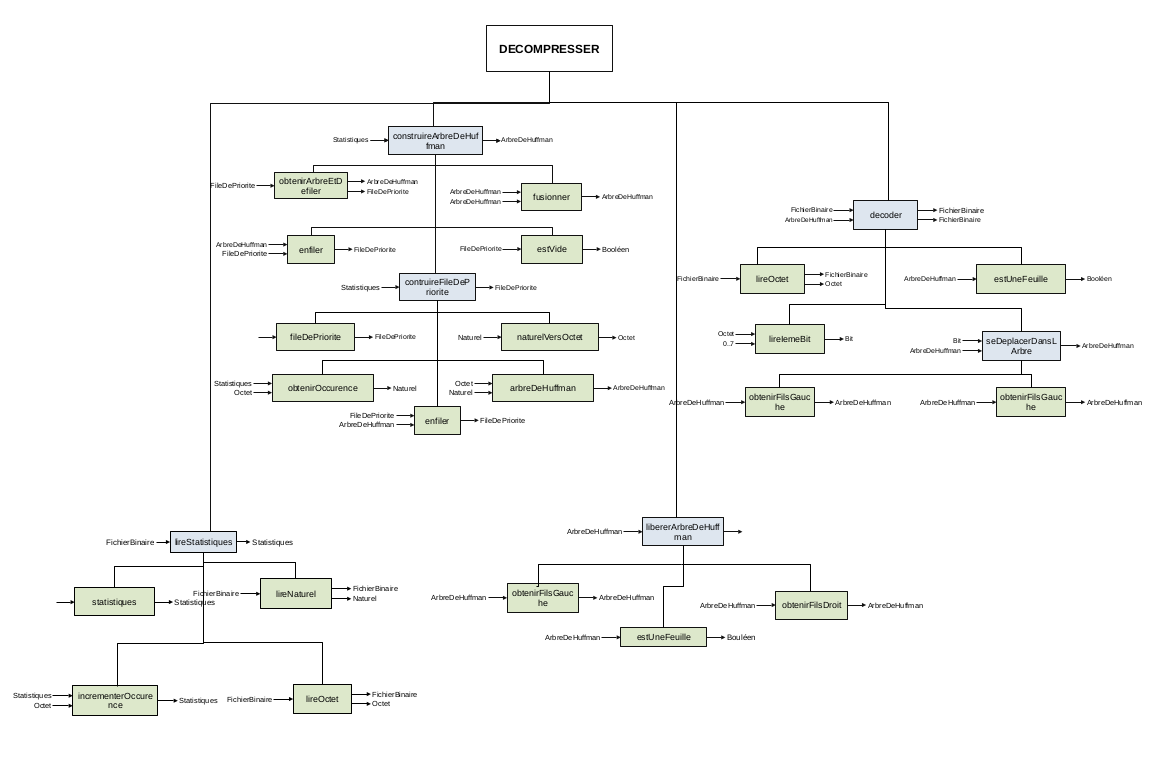
\includegraphics[width=1.1\textwidth]{decompresser.png}
        \caption{Analyse descendante de la décompression}
        \label{fig:exemple}
    \end{figure}
    
\newpage
\section{Conception Préliminaire}
    \begin{algorithme}
    \signatureFonction{lireStatistiques}{fb : \fichierbinaire}{\statistiques}{estOuvert(fb) et (mode(fb) $=$ lecture)}
\end{algorithme}
    \begin{algorithme}
    \signatureFonction{construireFileDePriorite}{s : \statistiques}{\filedepriorite}{}
\end{algorithme}
    \begin{algorithme}
    \signatureFonction{construireArbreDeHufmman}{s : \statistiques}{\arbredehuffman}{}
\end{algorithme}
    \begin{algorithme}
    \signatureProcedure{seDeplacerDansLArbre}
{\paramEntree{bit : \bit, a1 : \arbredehuffman}, \paramSortie{a2 : \arbredehuffman}}{}
\end{algorithme}
    \begin{algorithme}
    \signatureProcedure{decoder}
{\paramEntree{a : \arbredehuffman, longueur : \naturel}, \paramEntreeSortie{fb1 : \fichierbinaire, fb2 : \fichierbinaire}}{estOuvert(fb1) et (mode(fb1) $=$ lecture) et estOuvert(fb2) et (mode(fb2) $=$ écriture)}
\end{algorithme}
    \begin{algorithme}
    \signatureProcedure{decompresser}{\paramEntreeSortie{fCompresse : \fichierbinaire}, \paramSortie{fDecompresse : \fichierbinaire}}{}
\end{algorithme}

\newpage
\section{Conception Détaillée}
    \begin{algorithme}
    \fonction{lireStatistiques}{fb : \fichierbinaire}{\statistiques}{estOuvert(fb) et (mode(fb) $=$ lecture)}
    {n, i : \naturel , s : \statistiques}
    {
    	\affecter{s}{statistiques()}
    	\commentaire{La fonction lireStatistiques est utilisée quand le curseur est au bon endroit et l'on peut donc directement lire les statistiques qui sont des naturels}
    	\pour{i}{0}{255}{}
    	{
    		\instruction{lireNaturel(fb, n)}
        	\affecter{s[i]}{n}
    	}
    \retourner{s}
    }
\end{algorithme}
    \begin{algorithme}
    \fonction{construireFileDePriorite}{s : \statistiques}{\filedepriorite}{}
    {fdp : \filedepriorite, octet : \octet, occurence : \naturel}
    {
        \affecter{fdp}{fileDePriorite()}
        \pour{o}{ 0}{255}{}
        {
            \affecter{octet}{naturelVersOctet(o)}
            \affecter{occurence}{obtenirOccurence(s, octet)}
            \sialors{occurence > 0}{
                \instruction{enfiler(fdp, arbreDeHuffman(octet, occurence))}
            }
        }
        \retourner{fdp}
    }
\end{algorithme}
    \begin{algorithme}
	\fonction{construireArbreDeHuffman}{s : \statistiques}{\arbredehuffman}{}
	{fdp : \filedepriorite, dernierElement : \booleen, a1, a2, aFusion : \arbredehuffman}
    {
    	\affecter{fdp}{construireFileDePriorite(s)}
    	\affecter{dernierElement}{estVide(fdp)}
    	\tantque{non(dernierElement)}
    	{
    		\instruction{obtenirElementEtDefiler(fdp, a1)}
    		\sialorssinon{estVide(fdp)}
    		{
    			\affecter{dernierElement}{VRAI}
    		}
    		{
    			\instruction{obtenirElementEtDefiler(fdp, a2)}
    			\affecter{aFusion}{fusionner(a1, a2)}
    			\instruction{enfiler(fdp, aFusion)}
    		}
    	}
    	}
    	\retourner{a1}
    }
\end{algorithme}
    \begin{algorithme}
    \procedure{seDeplacerDansLArbre}{\paramEntree{bit : bit}, \paramEntreeSortie{arbreCourant : ArbreDeHuffman}}{}{}
    {
        \sialors{bit = 0}
        {
            \affecter{arbreCourant}{obtenirFilsGauche(arbreCourant)}
        }
        \sialors{bit = 1}
        {
            \affecter{arbreCourant}{obtenirFilsDroit(arbreCourant)}
        }
    }
\end{algorithme}

    \begin{algorithme}
    \procedure{decoder}{\paramEntree{aHuff : \arbredehuffman, longueur : \naturel}, \paramEntreeSortie{fb1:\fichierbinaire, fb2 : \fichierbinaire}}{}{compteurOctetsDecodes : \naturel}
    {
       \affecter{aTemp}{aHuff}
       \affecter{compteurOctetsDecodes}{0}
       \tantque{compteurOctetsDecodes <= longueur}{
       		\affecter{OctetCourant}{lireOctet(fb1)}
       		\pour{i}{0}{7}{}
       		{
       			\affecter{Bit}{IemeBit(OctetCourant,i)}
       			\instruction{seDeplacerDansLArbre(bit,atemp)}
       			\sialors{estUneFeuille(atemp)}{
       				\affecter{octetDecodé}{obtenirOctet(aTemp)}
       				\instruction{écrireOctet(octetDecodé, fb2)}
       				\affecter{compteurOctetsDecodes}{compteurOctetsDecodes+1}
       				\affecter{aTemp}{aHuff}
       				}
       			}
       		}
    }
    
\end{algorithme}
    \begin{algorithme}
	\procedure{decompresser}{\paramEntreeSortie{fCompresse : \fichierbinaire}, \paramSortie{fDecompresse : \fichierbinaire}}
	{estOuvert(fCompresse) et (mode(fCompresse) $=$ lecture)}
	{i, id, longueur : \naturel, s : \statistiques, abh : \arbredehuffman, octetUnique : \octet}
    {
		\instruction{positionnerAuDebut(fCompresse)}
		\instruction{ouvrir(fDecompresse, ecriture)}
    	\instruction{lireNaturel(fCompresser, id)}
		\\
    	\commentaire{On vérifie si on retrouve bien notre identifiant (ici 1000 sous sa forme de naturel), si ce n'est pas le cas, on n'a pas a décompresser le fichier}
    	\sialors{id = 1000}{   
			\instruction{lireNaturel(fCompresser, longueur)}
			\\\commentaire{Cas particulier d'un fichier vide}
			\sialors{(longueur > 0)}{
				\instruction{lireStatistiques(fCompresser, s)}
				\instruction{construireArbreDeHuffman(s, abh)}
				\\\commentaire{Cas particulier d'un fichier contenant un seul octet (présent plusieurs fois ou non)}
				\sialorssinon{estUneFeuille(abh)}
				{
					\affecter{octetUnique}{octetVersNaturel(obtenirOctet(abh))}
					\pour{i}{1}{longueur}{}{
						\instruction{ecrireOctet(fDecompresse, octetUnique)}
					}
				}
				{
					\instruction{decoder(abh, longueur, fCompresse, fDecompresse)}
				}
				\instruction{liberer(abh)}
			}
    	}
		\instruction{fermer(fDecompresse)}
    }
\end{algorithme}

    \chapter{Développement}
    \section{Fichiers d'en-tête}
    \subsection{TAD Octet}
        \inputminted[breaklines,fontfamily=fi4]{c}{../include/octet.h}
    \subsection{TAD Statistiques}
        \inputminted[breaklines,fontfamily=fi4]{c}{../include/statistiques.h}
    \subsection{TAD FileDePriorite}
        \inputminted[breaklines,fontfamily=fi4]{c}{../include/fileDePrioriteDArbreDeHuffman.h}
    \subsection{TAD ArbreDeHuffman}
        \inputminted[breaklines,fontfamily=fi4]{c}{../include/arbreDeHuffman.h}
    \subsection{TAD CodeBinaire}
        \inputminted[breaklines,fontfamily=fi4]{c}{../include/codeBinaire.h}
    \subsection{TAD TableDeCodage}
        \inputminted[breaklines,fontfamily=fi4]{c}{../include/tableDeCodage.h}
    \subsection{Construction de l'arbre de Huffman}
        \inputminted[breaklines,fontfamily=fi4]{c}{../include/construireArbreDeHuffman.h}
    \subsection{Compression}
        \inputminted[breaklines,fontfamily=fi4]{c}{../include/compression.h}
    \subsection{Décompression}
        \inputminted[breaklines,fontfamily=fi4]{c}{../include/decompression.h} 

\newpage
\section{Code source}
    \subsection{TAD Octet}
        \inputminted[breaklines,fontfamily=fi4]{c}{../src/octet.c}
    \subsection{TAD Statistiques}
        \inputminted[breaklines,fontfamily=fi4]{c}{../src/statistiques.c}
    \subsection{TAD FileDePriorite}
        \inputminted[breaklines,fontfamily=fi4]{c}{../src/fileDePrioriteDArbreDeHuffman.c}
    \subsection{TAD ArbreDeHuffman}
        \inputminted[breaklines,fontfamily=fi4]{c}{../src/arbreDeHuffman.c}
    \subsection{TAD CodeBinaire}
        \inputminted[breaklines,fontfamily=fi4]{c}{../src/codeBinaire.c}
    \subsection{TAD TableDeCodage}
        \inputminted[breaklines,fontfamily=fi4]{c}{../src/tableDeCodage.c}
    \subsection{Fonctions communes à la compression et à la décompression}
        \inputminted[breaklines,fontfamily=fi4]{c}{../src/construireArbreDeHuffman.c}
    \subsection{Compression}
        \inputminted[breaklines,fontfamily=fi4]{c}{../src/compression.c}
    \subsection{Décompression}
        \inputminted[breaklines,fontfamily=fi4]{c}{../src/decompression.c} 
    \subsection{Programme principal}
        \inputminted[breaklines,fontfamily=fi4]{c}{../src/main.c}

\newpage
\section{Tests unitaires}
    \subsection{Tests des TADs}
        \inputminted[breaklines,fontfamily=fi4]{c}{../src/testsTADs.c}
    \subsection{Tests des fonctions métier}
        \inputminted[breaklines,fontfamily=fi4]{c}{../src/testsFonctionsMetier.c}

    \chapter{Travail de Groupe}
        \section{Distribution des tâches}
    \begin{table}[ht]
    \centering
    \begin{tabular}{|c|c|>{\centering\arraybackslash}p{1.5cm}|>{\centering\arraybackslash}p{1.5cm}|>{\centering\arraybackslash}p{1.5cm}|>{\centering\arraybackslash}p{1.5cm}|}
        \cline{3-6}
        \multicolumn{2}{c|}{} & Taoba & Thomas & Ali & Mathis \\
        \hline
        \multirow{7}{*}{Analyse (TAD)}
        & CodeBinaire & & & $\times$ & \\
        \cline{2-6}
        & Octet & & & & $\times$ \\
        \cline{2-6}
        & Statistiques & $\times$ & & & \\ 
        \cline{2-6}
        & ArbreDeHuffman & & $\times$ & & \\
        \cline{2-6}
        & FileDePriorité & & $\times$ & & \\
        \cline{2-6}
        & TableDeCodage & & & & $\times$ \\
        \hline
        \multirow{7}{*}{CP}
        & Code Binaire & & & & $\times$ \\
        \cline{2-6}
        & Octet & & $\times$ & & \\
        \cline{2-6}
        & Statistiques & & $\times$ & & \\
        \cline{2-6}
        & ArbreDeHuffman & $\times$ & & & \\
        \cline{2-6}
        & FileDePriorité & & & & $\times$ \\
        \cline{2-6}
        & TableDeCodage & & & $\times$ & \\
        \hline
        \multirow{7}{*}{CD}
        & CodeBinaire & $\times$ & & & \\
        \cline{2-6}
        & Octet & $\times$ & & & \\
        \cline{2-6}
        & Statistiques & & & & $\times$ \\
        \cline{2-6}
        & ArbreDeHuffman & & & $\times$ & $\times$ \\
        \cline{2-6}
        & FileDePriorité & & & $\times$ & \\
        \cline{2-6}
        & TableDeCodage & & $\times$ & & \\
        \hline
        \multirow{7}{*}{Dev}
        & CodeBinaire & & $\times$ & & \\
        \cline{2-6}
        & Octet & & & $\times$ & \\
        \cline{2-6}
        & Statistiques & & $\times$ & & \\
        \cline{2-6}
        & ArbreDeHuffman & & & $\times$ & $\times$ \\
        \cline{2-6}
        & FileDePriorité & & & & $\times$ \\
        \cline{2-6}
        & TableDeCodage & $\times$ & & & \\
        \hline
        \multirow{7}{*}{Tests unitaires}
        & CodeBinaire & & $\times$ & & \\
        \cline{2-6}
        & Octet & & & $\times$ & \\
        \cline{2-6}
        & Statistiques & & $\times$ & & \\
        \cline{2-6}
        & ArbreDeHuffman & $\times$ & & & \\
        \cline{2-6}
        & FileDePriorité & $\times$ & & & \\
        \cline{2-6}
        & TableDeCodage & & & & $\times$ \\
        \hline
    \end{tabular}
    \caption{Tableau des tâches des TADs}
  \end{table}  
 
 
 \begin{table}[ht]
    \centering
    \begin{tabular}{|c|c|>{\centering\arraybackslash}p{1.5cm}|>{\centering\arraybackslash}p{1.5cm}|>{\centering\arraybackslash}p{1.5cm}|>{\centering\arraybackslash}p{1.5cm}|}
        \cline{3-6}
        \multicolumn{2}{c|}{} & Taoba & Thomas & Ali & Mathis \\
        \hline
        \multirow{8}{*}{Analyse}
        & obtenirStatistiqueEtTailleFichier & & & $\times$ & $\times$ \\
        \cline{2-6}
        & ecrire\{Statistiques,Identifiant,Taille\} &  & & $\times$ & $\times$ \\ 
        \cline{2-6}
        & construireFileDePriorité & $\times$ & $\times$ & $\times$ & $\times$ \\
        \cline{2-6}
        & construireArbreDeHuffman & $\times$ & $\times$ & $\times$ & $\times$ \\
        \cline{2-6}
        & codeBinaireEnOctet & & & $\times$ & $\times$ \\
        \cline{2-6}
        & obtenirTableDeCodage & & & $\times$ & $\times$ \\
        \cline{2-6}
        & concatenerCodeBinaireDansFichier & & & $\times$ & $\times$ \\
        \cline{2-6}
        & encoder & & & $\times$ & $\times$ \\
        \cline{2-6}
        & compresser & & & $\times$ & $\times$ \\
        \hline
        \multirow{8}{*}{CP}
        & obtenirStatistiqueEtTailleFichier & $\times$ & & &  \\
        \cline{2-6}
        & ecrire\{Statistiques,Identifiant,Taille\} & & $\times$ & & \\ 
        \cline{2-6}
        & construireFileDePriorité & $\times$ & & &  \\
        \cline{2-6}
        & construireArbreDeHuffman & & & $\times$ & \\
        \cline{2-6}
        & obtenirTableDeCodage & $\times$ & & &  \\
        \cline{2-6}
        & codeBinaireEnOctet & & $\times$& & \\
        \cline{2-6}
        & concatenerCodeBinaireDansFichier & & $\times$ & & \\
        \cline{2-6}
        & encoder & & $\times$ & & \\
        \cline{2-6}
        & compresser & $\times$ & & & \\
        \hline
        \multirow{8}{*}{CD}
        & obtenirStatistiqueEtTailleFichier & & $\times$ & & \\
        \cline{2-6}
        & ecrire\{Statistiques,Identifiant,Taille\} & $\times$ & & & \\ 
        \cline{2-6}
        & construireFileDePriorité & & $\times$ & &\\
        \cline{2-6}
        & construireArbreDeHuffman & & & $\times$ & \\
        \cline{2-6}
        & obtenirTableDeCodage & & $\times$ & & \\
        \cline{2-6}
        & codeBinaireEnOctet & $\times$ & & & \\
        \cline{2-6}
        & concatenerCodeBinaireDansFichier & $\times$ & $\times$ & & \\
        \cline{2-6}
        & encoder & $\times$ & & & \\
        \cline{2-6}
        & compresser & & $\times$ & &\\
        \hline
        \multirow{8}{*}{Dev}
        & obtenirStatistiqueEtTailleFichier & $\times$ & & & \\
        \cline{2-6}
        & ecrire\{Statistiques,Identifiant,Taille\} & & $\times$ & & \\ 
        \cline{2-6}
        & construireFileDePriorité & $\times$ & & & \\
        \cline{2-6}
        & construireArbreDeHuffman & & & & $\times$ \\
        \cline{2-6}
        & obtenirTableDeCodage & $\times$ & & & \\
        \cline{2-6}
        & codeBinaireEnOctet & & $\times$ & & \\
        \cline{2-6}
        & concatenerCodeBinaireDansFichier & & $\times$ & & \\
        \cline{2-6}
        & encoder & & $\times$ & & \\
        \cline{2-6}
        & compresser & $\times$ & & & \\
        \hline
        \multirow{8}{*}{Tests Unitaires}
        & obtenirStatistiqueEtTailleFichier & & $\times$ & & \\
        \cline{2-6}
        & ecrire\{Statistiques,Identifiant,Taille\} & $\times$ & & & \\ 
        \cline{2-6}
        & construireFileDePriorité & & $\times$ & & \\
        \cline{2-6}
        & construireArbreDeHuffman & & $\times$ & & \\
        \cline{2-6}
        & obtenirTableDeCodage & & $\times$ & & \\
        \cline{2-6}
        & codeBinaireEnOctet & $\times$ & & & \\
        \cline{2-6}
        & concatenerCodeBinaireDansFichier & $\times$ & & & \\
        \cline{2-6}
        & encoder & $\times$ & & & \\
        \cline{2-6}
        & compresser & & $\times$ & & \\
        \hline
    \end{tabular}
    \caption{Tableau des tâches de la compression}
  \end{table}  
 
 
 \begin{table}[ht]
    \centering
    \begin{tabular}{|c|c|>{\centering\arraybackslash}p{1.5cm}|>{\centering\arraybackslash}p{1.5cm}|>{\centering\arraybackslash}p{1.5cm}|>{\centering\arraybackslash}p{1.5cm}|}
        \cline{3-6}
        \multicolumn{2}{c|}{} & Taoba & Thomas & Ali & Mathis \\
        \hline
        \multirow{6}{*}{Analyse}
        & lireStatistiques & $\times$ & $\times$ & & \\
        \cline{2-6}
        & construireFileDePriorité & $\times$ & $\times$ & $\times$ & $\times$ \\
        \cline{2-6}
        & construireArbreDeHuffman & $\times$ & $\times$ & $\times$ & $\times$ \\
        \cline{2-6}
        & seDeplacerDansLArbre & $\times$ & $\times$ & & \\
        \cline{2-6}
        & decoder & $\times$ & $\times$ & & \\
        \cline{2-6}
        & decompresser & $\times$ & $\times$ & & \\ 
        \hline
         \multirow{6}{*}{CP}
        & lireStatistiques & & & $\times$ & \\
        \cline{2-6}
        & construireFileDePriorité & $\times$ & & &  \\
        \cline{2-6}
        & construireArbreDeHuffman & & & $\times$ & \\
        \cline{2-6}
        & seDeplacerDansLArbre & & & & $\times$ \\
        \cline{2-6}
        & decoder & & & & $\times$ \\
        \cline{2-6}
        & decompresser & & & $\times$ & \\ 
        \hline
        \multirow{6}{*}{CD}
        & lireStatistiques & & & & $\times$ \\
        \cline{2-6}
        & construireFileDePriorité & & $\times$ & & \\
        \cline{2-6}
        & construireArbreDeHuffman & & & & $\times$ \\
        \cline{2-6}
        & seDeplacerDansLArbre & & & $\times$ & \\
        \cline{2-6}
        & decoder & & & $\times$ & \\
        \cline{2-6}
        & decompresser & & & & $\times$ \\ 
        \hline
        \multirow{6}{*}{Dev}
        & lireStatistiques & & & $\times$ & \\
        \cline{2-6}
        & construireFileDePriorité & $\times$ & & & \\
        \cline{2-6}
        & construireArbreDeHuffman & & & $\times$ & \\
        \cline{2-6}
        & seDeplacerDansLArbre & & & & $\times$ \\
        \cline{2-6}
        & decoder & & & & $\times$ \\
        \cline{2-6}
        & decompresser & & & & $\times$ \\ 
        \hline
        \multirow{6}{*}{Tests Unitaires}
        & lireStatistiques & & & $\times$ & \\
        \cline{2-6}
        & construireFileDePriorité & & $\times$ & & \\
        \cline{2-6}
        & construireArbreDeHuffman & & $\times$ & & \\
        \cline{2-6}
        & seDeplacerDansLArbre & & & & $\times$ \\
        \cline{2-6}
        & decoder & & & & $\times$ \\
        \cline{2-6}
        & decompresser & & & $\times$ & \\ 
        \hline
    \end{tabular}
    \caption{Tableau des tâches de la décompression}
  \end{table}

    \chapter{Conclusion}
        
Dans ce projet, nous avons élaboré un algorithme de compression sans perte basé sur un arbre de Huffman, en suivant une conception en quatre phase:

    La première phase a consisté en la conception des TADs et des analyses descendantes nécessaires à la mise en place de notre compresseur Huffman.

    Ensuite, nous avons réalisé la conception préliminaire de nos fonctions et procédures, jetant ainsi les bases de l'implémentation.

    La troisième phase a été consacrée à la conception détaillée, où nous avons approfondi chaque aspect de l'algorithme, clarifiant les spécifications et les interactions entre les différentes parties du code.

    Enfin, nous avons procédé à l'implémentation du code en langage C et à la réalisation des tests unitaires pour évaluer le fonctionnement des algorithmes.

Les résultats des tests, principalement réalisés sur des fichiers textes, démontrent l'efficacité de notre algorithme en termes de réduction de la taille des données, tout en préservant l'intégrité des informations d'origine.

L'utilisation d'une compression sans perte de données pour les fichiers texte est cruciale, car elle garantit la conservation du sens du texte d'origine. Nous aurions également pu explorer des méthodes de compression par perte de données et discuter de leur utilisation sur des fichiers audio ou images sur lesquels notre algorithme ne fonctionne pas étant des fichiers déjà compressé.

Le travail de groupe a été essentiel à la réussite de ce projet. Nous avons pu partager les tâches et les responsabilités, bénéficier des compétences et des connaissances des autres membres du groupe, et résoudre les problèmes de manière collective.

Concernant les perspectives d'amélioration, notre algorithme de compression pourrait être optimisé de différentes manières. Par exemple, l'utilisation d'un autre algorithme pour la construction de l'arbre de Huffman ou l'exploration de techniques de compression plus avancées telles que la compression par blocs ou la compression par transformation.





\end{document}
